%% bare_conf.tex
%% V1.3
%% 2007/01/11
%% by Michael Shell
%% See:
%% http://www.michaelshell.org/
%% for current contact information.
%%
%% This is a skeleton file demonstrating the use of IEEEtran.cls
%% (requires IEEEtran.cls version 1.7 or later) with an IEEE conference paper.
%%
%% Support sites:
%% http://www.michaelshell.org/tex/ieeetran/
%% http://www.ctan.org/tex-archive/macros/latex/contrib/IEEEtran/
%% and
%% http://www.ieee.org/

%%*************************************************************************
%% Legal Notice:
%% This code is offered as-is without any warranty either expressed or
%% implied; without even the implied warranty of MERCHANTABILITY or
%% FITNESS FOR A PARTICULAR PURPOSE! 
%% User assumes all risk.
%% In no event shall IEEE or any contributor to this code be liable for
%% any damages or losses, including, but not limited to, incidental,
%% consequential, or any other damages, resulting from the use or misuse
%% of any information contained here.
%%
%% All comments are the opinions of their respective authors and are not
%% necessarily endorsed by the IEEE.
%%
%% This work is distributed under the LaTeX Project Public License (LPPL)
%% ( http://www.latex-project.org/ ) version 1.3, and may be freely used,
%% distributed and modified. A copy of the LPPL, version 1.3, is included
%% in the base LaTeX documentation of all distributions of LaTeX released
%% 2003/12/01 or later.
%% Retain all contribution notices and credits.
%% ** Modified files should be clearly indicated as such, including  **
%% ** renaming them and changing author support contact information. **
%%
%% File list of work: IEEEtran.cls, IEEEtran_HOWTO.pdf, bare_adv.tex,
%%                    bare_conf.tex, bare_jrnl.tex, bare_jrnl_compsoc.tex
%%*************************************************************************

% *** Authors should verify (and, if needed, correct) their LaTeX system  ***
% *** with the testflow diagnostic prior to trusting their LaTeX platform ***
% *** with production work. IEEE's font choices can trigger bugs that do  ***
% *** not appear when using other class files.                            ***
% The testflow support page is at:
% http://www.michaelshell.org/tex/testflow/



% Note that the a4paper option is mainly intended so that authors in
% countries using A4 can easily print to A4 and see how their papers will
% look in print - the typesetting of the document will not typically be
% affected with changes in paper size (but the bottom and side margins will).
% Use the testflow package mentioned above to verify correct handling of
% both paper sizes by the user's LaTeX system.
%
% Also note that the "draftcls" or "draftclsnofoot", not "draft", option
% should be used if it is desired that the figures are to be displayed in
% draft mode.
%
\documentclass[10pt, conference, compsocconf, english]{IEEEtran}
%\documentclass[10pt, conference, compsocconf]{IEEEtran}
% Add the compsocconf option for Computer Society conferences.
%
% If IEEEtran.cls has not been installed into the LaTeX system files,
% manually specify the path to it like:
% \documentclass[conference]{../sty/IEEEtran}





% Some very useful LaTeX packages include:
% (uncomment the ones you want to load)


% *** MISC UTILITY PACKAGES ***
%
%\usepackage{ifpdf}
% Heiko Oberdiek's ifpdf.sty is very useful if you need conditional
% compilation based on whether the output is pdf or dvi.
% usage:
% \ifpdf
%   % pdf code
% \else
%   % dvi code
% \fi
% The latest version of ifpdf.sty can be obtained from:
% http://www.ctan.org/tex-archive/macros/latex/contrib/oberdiek/
% Also, note that IEEEtran.cls V1.7 and later provides a builtin
% \ifCLASSINFOpdf conditional that works the same way.
% When switching from latex to pdflatex and vice-versa, the compiler may
% have to be run twice to clear warning/error messages.






% *** CITATION PACKAGES ***
%
%\usepackage{cite}
% cite.sty was written by Donald Arseneau
% V1.6 and later of IEEEtran pre-defines the format of the cite.sty package
% \cite{} output to follow that of IEEE. Loading the cite package will
% result in citation numbers being automatically sorted and properly
% "compressed/ranged". e.g., [1], [9], [2], [7], [5], [6] without using
% cite.sty will become [1], [2], [5]--[7], [9] using cite.sty. cite.sty's
% \cite will automatically add leading space, if needed. Use cite.sty's
% noadjust option (cite.sty V3.8 and later) if you want to turn this off.
% cite.sty is already installed on most LaTeX systems. Be sure and use
% version 4.0 (2003-05-27) and later if using hyperref.sty. cite.sty does
% not currently provide for hyperlinked citations.
% The latest version can be obtained at:
% http://www.ctan.org/tex-archive/macros/latex/contrib/cite/
% The documentation is contained in the cite.sty file itself.






% *** GRAPHICS RELATED PACKAGES ***
%
\ifCLASSINFOpdf
  % \usepackage[pdftex]{graphicx}
  % declare the path(s) where your graphic files are
  % \graphicspath{{../pdf/}{../jpeg/}}
  % and their extensions so you won't have to specify these with
  % every instance of \includegraphics
  % \DeclareGraphicsExtensions{.pdf,.jpeg,.png}
\else
  % or other class option (dvipsone, dvipdf, if not using dvips). graphicx
  % will default to the driver specified in the system graphics.cfg if no
  % driver is specified.
  % \usepackage[dvips]{graphicx}
  % declare the path(s) where your graphic files are
  % \graphicspath{{../eps/}}
  % and their extensions so you won't have to specify these with
  % every instance of \includegraphics
  % \DeclareGraphicsExtensions{.eps}
\fi
% graphicx was written by David Carlisle and Sebastian Rahtz. It is
% required if you want graphics, photos, etc. graphicx.sty is already
% installed on most LaTeX systems. The latest version and documentation can
% be obtained at: 
% http://www.ctan.org/tex-archive/macros/latex/required/graphics/
% Another good source of documentation is "Using Imported Graphics in
% LaTeX2e" by Keith Reckdahl which can be found as epslatex.ps or
% epslatex.pdf at: http://www.ctan.org/tex-archive/info/
%
% latex, and pdflatex in dvi mode, support graphics in encapsulated
% postscript (.eps) format. pdflatex in pdf mode supports graphics
% in .pdf, .jpeg, .png and .mps (metapost) formats. Users should ensure
% that all non-photo figures use a vector format (.eps, .pdf, .mps) and
% not a bitmapped formats (.jpeg, .png). IEEE frowns on bitmapped formats
% which can result in "jaggedy"/blurry rendering of lines and letters as
% well as large increases in file sizes.
%
% You can find documentation about the pdfTeX application at:
% http://www.tug.org/applications/pdftex





% *** MATH PACKAGES ***
%
%\usepackage[cmex10]{amsmath}
% A popular package from the American Mathematical Society that provides
% many useful and powerful commands for dealing with mathematics. If using
% it, be sure to load this package with the cmex10 option to ensure that
% only type 1 fonts will utilized at all point sizes. Without this option,
% it is possible that some math symbols, particularly those within
% footnotes, will be rendered in bitmap form which will result in a
% document that can not be IEEE Xplore compliant!
%
% Also, note that the amsmath package sets \interdisplaylinepenalty to 10000
% thus preventing page breaks from occurring within multiline equations. Use:
%\interdisplaylinepenalty=2500
% after loading amsmath to restore such page breaks as IEEEtran.cls normally
% does. amsmath.sty is already installed on most LaTeX systems. The latest
% version and documentation can be obtained at:
% http://www.ctan.org/tex-archive/macros/latex/required/amslatex/math/





% *** SPECIALIZED LIST PACKAGES ***
%
%\usepackage{algorithmic}
% algorithmic.sty was written by Peter Williams and Rogerio Brito.
% This package provides an algorithmic environment fo describing algorithms.
% You can use the algorithmic environment in-text or within a figure
% environment to provide for a floating algorithm. Do NOT use the algorithm
% floating environment provided by algorithm.sty (by the same authors) or
% algorithm2e.sty (by Christophe Fiorio) as IEEE does not use dedicated
% algorithm float types and packages that provide these will not provide
% correct IEEE style captions. The latest version and documentation of
% algorithmic.sty can be obtained at:
% http://www.ctan.org/tex-archive/macros/latex/contrib/algorithms/
% There is also a support site at:
% http://algorithms.berlios.de/index.html
% Also of interest may be the (relatively newer and more customizable)
% algorithmicx.sty package by Szasz Janos:
% http://www.ctan.org/tex-archive/macros/latex/contrib/algorithmicx/




% *** ALIGNMENT PACKAGES ***
%
%\usepackage{array}
% Frank Mittelbach's and David Carlisle's array.sty patches and improves
% the standard LaTeX2e array and tabular environments to provide better
% appearance and additional user controls. As the default LaTeX2e table
% generation code is lacking to the point of almost being broken with
% respect to the quality of the end results, all users are strongly
% advised to use an enhanced (at the very least that provided by array.sty)
% set of table tools. array.sty is already installed on most systems. The
% latest version and documentation can be obtained at:
% http://www.ctan.org/tex-archive/macros/latex/required/tools/


%\usepackage{mdwmath}
%\usepackage{mdwtab}
% Also highly recommended is Mark Wooding's extremely powerful MDW tools,
% especially mdwmath.sty and mdwtab.sty which are used to format equations
% and tables, respectively. The MDWtools set is already installed on most
% LaTeX systems. The lastest version and documentation is available at:
% http://www.ctan.org/tex-archive/macros/latex/contrib/mdwtools/


% IEEEtran contains the IEEEeqnarray family of commands that can be used to
% generate multiline equations as well as matrices, tables, etc., of high
% quality.


%\usepackage{eqparbox}
% Also of notable interest is Scott Pakin's eqparbox package for creating
% (automatically sized) equal width boxes - aka "natural width parboxes".
% Available at:
% http://www.ctan.org/tex-archive/macros/latex/contrib/eqparbox/





% *** SUBFIGURE PACKAGES ***
%\usepackage[tight,footnotesize]{subfigure}
% subfigure.sty was written by Steven Douglas Cochran. This package makes it
% easy to put subfigures in your figures. e.g., "Figure 1a and 1b". For IEEE
% work, it is a good idea to load it with the tight package option to reduce
% the amount of white space around the subfigures. subfigure.sty is already
% installed on most LaTeX systems. The latest version and documentation can
% be obtained at:
% http://www.ctan.org/tex-archive/obsolete/macros/latex/contrib/subfigure/
% subfigure.sty has been superceeded by subfig.sty.



%\usepackage[caption=false]{caption}
%\usepackage[font=footnotesize]{subfig}
% subfig.sty, also written by Steven Douglas Cochran, is the modern
% replacement for subfigure.sty. However, subfig.sty requires and
% automatically loads Axel Sommerfeldt's caption.sty which will override
% IEEEtran.cls handling of captions and this will result in nonIEEE style
% figure/table captions. To prevent this problem, be sure and preload
% caption.sty with its "caption=false" package option. This is will preserve
% IEEEtran.cls handing of captions. Version 1.3 (2005/06/28) and later 
% (recommended due to many improvements over 1.2) of subfig.sty supports
% the caption=false option directly:
%\usepackage[caption=false,font=footnotesize]{subfig}
%
% The latest version and documentation can be obtained at:
% http://www.ctan.org/tex-archive/macros/latex/contrib/subfig/
% The latest version and documentation of caption.sty can be obtained at:
% http://www.ctan.org/tex-archive/macros/latex/contrib/caption/




% *** FLOAT PACKAGES ***
%
%\usepackage{fixltx2e}
% fixltx2e, the successor to the earlier fix2col.sty, was written by
% Frank Mittelbach and David Carlisle. This package corrects a few problems
% in the LaTeX2e kernel, the most notable of which is that in current
% LaTeX2e releases, the ordering of single and double column floats is not
% guaranteed to be preserved. Thus, an unpatched LaTeX2e can allow a
% single column figure to be placed prior to an earlier double column
% figure. The latest version and documentation can be found at:
% http://www.ctan.org/tex-archive/macros/latex/base/



%\usepackage{stfloats}
% stfloats.sty was written by Sigitas Tolusis. This package gives LaTeX2e
% the ability to do double column floats at the bottom of the page as well
% as the top. (e.g., "\begin{figure*}[!b]" is not normally possible in
% LaTeX2e). It also provides a command:
%\fnbelowfloat
% to enable the placement of footnotes below bottom floats (the standard
% LaTeX2e kernel puts them above bottom floats). This is an invasive package
% which rewrites many portions of the LaTeX2e float routines. It may not work
% with other packages that modify the LaTeX2e float routines. The latest
% version and documentation can be obtained at:
% http://www.ctan.org/tex-archive/macros/latex/contrib/sttools/
% Documentation is contained in the stfloats.sty comments as well as in the
% presfull.pdf file. Do not use the stfloats baselinefloat ability as IEEE
% does not allow \baselineskip to stretch. Authors submitting work to the
% IEEE should note that IEEE rarely uses double column equations and
% that authors should try to avoid such use. Do not be tempted to use the
% cuted.sty or midfloat.sty packages (also by Sigitas Tolusis) as IEEE does
% not format its papers in such ways.





% *** PDF, URL AND HYPERLINK PACKAGES ***
%
\usepackage{url}
% url.sty was written by Donald Arseneau. It provides better support for
% handling and breaking URLs. url.sty is already installed on most LaTeX
% systems. The latest version can be obtained at:
% http://www.ctan.org/tex-archive/macros/latex/contrib/misc/
% Read the url.sty source comments for usage information. Basically,
% \url{my_url_here}.

\usepackage[sort&compress]{natbib}
\usepackage{graphicx}
\usepackage[figuresright]{rotating}
\graphicspath{{./figures/}}
\usepackage{pifont}
\newcommand{\cmark}{\ding{51}}%
\newcommand{\xmark}{\ding{55}}%

\usepackage[T1]{fontenc}
\usepackage[utf8]{inputenc}
\usepackage{babel}



\usepackage[table,xcdraw]{xcolor}
\usepackage{graphicx}
%\usepackage[ansinew]{inputenc}
%\usepackage{times}
\usepackage{setspace}
\usepackage{xspace}
\usepackage{float}
\usepackage{color}
\usepackage{colortbl}
\usepackage{verbatim}
\usepackage{textfit}
\usepackage{longtable}
\usepackage{multirow}
\usepackage{booktabs}
\usepackage{alltt}
\usepackage[T1]{fontenc}
%\usepackage[verbose,left=30mm,right=20mm,top=30mm,bottom=30mm]{geometry}
\usepackage{ae}
%\usepackage{fancyhdr}
\usepackage{fancybox}
\usepackage{multicol}
\usepackage{listings}
%\usepackage{subfigure}
\usepackage{amsfonts}
\usepackage{placeins}
\usepackage{url}
\usepackage{color}

%\usepackage{hyperref}
%\hypersetup{pdfborder=false}

%% correct bad hyphenation here
%\hyphenation{op-tical net-works semi-conduc-tor}


\begin{document}
%
% paper title
\title{Evolving an M-learning Software Product Line in an Industry Practitioner Perspective}

%\author{\IEEEauthorblockN{Anderson S. Marcolino, Ellen F. Barbosa}
%\IEEEauthorblockA{Institute of Science and Computational Mathematics -- University of S\~ao Paulo (ICMC--USP)\\
%S\~ao Carlos (SP), Brazil\\
%email: andersonmarcolino@gmail.com, francine@icmc.usp.br}
%
%}


% conference papers do not typically use \thanks and this command
% is locked out in conference mode. If really needed, such as for
% the acknowledgment of grants, issue a \IEEEoverridecommandlockouts
% after \documentclass

% for over three affiliations, or if they all won't fit within the width
% of the page, use this alternative format:
% 
%\author{\IEEEauthorblockN{Michael Shell\IEEEauthorrefmark{1},
%Homer Simpson\IEEEauthorrefmark{2},
%James Kirk\IEEEauthorrefmark{3}, 
%Montgomery Scott\IEEEauthorrefmark{3} and
%Eldon Tyrell\IEEEauthorrefmark{4}}
%\IEEEauthorblockA{\IEEEauthorrefmark{1}School of Electrical and Computer Engineering\\
%Georgia Institute of Technology,
%Atlanta, Georgia 30332--0250\\ Email: see http://www.michaelshell.org/contact.html}
%\IEEEauthorblockA{\IEEEauthorrefmark{2}Twentieth Century Fox, Springfield, USA\\
%Email: homer@thesimpsons.com}
%\IEEEauthorblockA{\IEEEauthorrefmark{3}Starfleet Academy, San Francisco, California 96678-2391\\
%Telephone: (800) 555--1212, Fax: (888) 555--1212}
%\IEEEauthorblockA{\IEEEauthorrefmark{4}Tyrell Inc., 123 Replicant Street, Los Angeles, California 90210--4321}}

% use for special paper notices
%\IEEEspecialpapernotice{(Invited Paper)}



% make the title area
\maketitle

%---------------------------------------
\begin{abstract}
The development of software that unifies the expertise from industry with theoretical techniques from academia may providing better and more quality results, with high level of reuse and lower costs. In this perspective, this paper integrates industry practice with academic research to evolve a software product line (SPL) for the development of mobile applications for the teaching of programming. The proposed SPL was evaluated in a previous study and, as a result, we noticed a lack in the integration of practitioners in the performed evaluation. Furthermore, as the set of features identified for the definition of the SPL scope is very broad, there is a need for adopting strategies that can reduce efforts in their development process. In this perspective, experts in development were considered in our research to allow: (i) the evaluation of the SPL conceptual architecture, (ii) the evolution of the SPL architecture, and (iii) the support in modeling of the diagrams that will be considered in implementation of both domain and test realization. The performed analyses provided discussions about: (i) the decisions taken, (ii) the new models of the SPL architecture evolved, (iii) the strategies and techniques adopted to conduct the implementation of each features, and (iv) lessons learned. At the end, considerations about the integration of practical and theoretical perspectives and future work are argued as well.
\end{abstract}
%---------------------------------------
%
%\begin{IEEEkeywords}
%	software product line engineering; mobile learning application; teaching of programming; architecture.
%\end{IEEEkeywords}

%---------------------------------------

% For peer review papers, you can put extra information on the cover
% page as needed:
% \ifCLASSOPTIONpeerreview
% \begin{center} \bfseries EDICS Category: 3-BBND \end{center}
% \fi
%
% For peerreview papers, this IEEEtran command inserts a page break and
% creates the second title. It will be ignored for other modes.
\IEEEpeerreviewmaketitle


\section{Introduction}
\label{sec:introdcution}

The adoption of information and communication technologies (ICTs) and their learning modalities have providing significant changes on the educational process. Teachers have adopting such technologies as a supporting mechanism in the classroom and to promote the continuity of studies in the learners' houses. Mobile learning (m-learning) is one of these modalities. It enables through mobile devices the learning at anyplace and everywhere. Moreover, such devices are low-cost and are widely present in the routine of young, adult and elder worldwide, creating a propitious scenario for its adoption in the educational process for several domains \cite{marcolino_edu2015, marcolinoarcht2017}.

On the other hand, the development of educational software and applications can hinder the process of adoption of ICTs' based modalities, due to issues involved, i.e., introducing pedagogical and didactic features in the solutions for supporting both teachers and learners; and guarantee the low-cost of the development of software that really met the needs of teachers and educators. An example of educational domain that need to overcome several problems is the teaching of programming \cite{souza2015}.

The majority of applications in the teaching of programming domain supports informal learning and do not provide a good level of feedback \cite{marcolino_edu2015}. Informal learning is the process of learning which there is no support of a human mediator, such as a teacher or tutor. The application itself is responsible for providing feedback, which difficult its adoption since it do not support widely teachers in classroom. The feedback gave by the applications do not show exactly the students' limitations, consequently teachers still need to monitoring in person their students in the learning process, being the main mediator between content and the learners' difficulties. 


Additionally, the reduced mobile devices keyboards and the few use of sensors and touchscreen interactions may demotivated the learners to program in such platform. In this perspective, there is a need of researches that consider the adoption of interactions seen in applications of social network and games for providing better educational applications, besides to identifying the features that really fit as an real improvement of learning for this modality \cite{marcolino_edu2015}.


In this perspective, the software product line (SPL) approach was selected for supporting the creation of mobile learning applications for the teaching of programming. The several issues and concerns involved in the educational area and in learning applications can benefit themselves from this methodology, since the teachers have the power to decide which features they expect in the applications for supporting them in classrooms, e.g., through an SPL it is possible to select features of content and learning activities, or only activities, supported by one or more programming languages. Besides, the applications can integrate different means of interaction and formats of learning content and activities \cite{marcolino_spl2015, marcolinoarcht2017}. Marcolino and Barbosa \cite{marcolinoarcht2017} presented an SPL conceptual architecture, conducting the three first sub--processes from the SPLE (software product line engineering) \cite{6799220, pohl2005}: product management, domain requirements engineering and domain design. 


The conceptual model \cite{marcolinoarcht2017} was evaluated by 31 experts from academic area (software engineers, programming teachers, m-learning experts and mobile developers), suggesting the architecture design is feasible. To complete such domain design activities, this study aims at: (i) evolving the conceptual architecture in a industry practitioners perspective through a re-analysis of the evaluated architecture, (ii) discussing the proposed improvements based on pedagogical and didactic issues; (iii) representing the improved architecture with UML (Unified Modeling Language) and SMarty (Stereotype-based Management of Variability); and (iv) presenting technique and methodology adopted for the conduction of domain realisation and domain testing SPLE sub-processes.

The research contributes towards: (i) easing SPL adoption for the development of mobile learning applications; (ii) discussing new technologies for supporting a better integration and reuse of pedagogical and didactic features; and (iii) improving the approaches and frameworks adopted considering mainly variables as developers team and time available.


This paper is organized as follows. Section \ref{sec:background} presents the main concepts about m-learning and the teaching of programming, the proposed m-learning SPL and the SMarty approach. Section \ref{sec:spl_project} presents the evolution of the SPL conceptual architecture process. Section \ref{sec:spl_smarty} presents and discusses the architecture represented with UML and SMarty. Finally, Section \ref{sec:conclusions} presents the conclusions and perspectives for future work.





\section{Background}
\label{sec:background}



\subsection{M-learning and the Teaching of Programming}

Mobile devices can be used for fun, entertainment, communication and learning, among many other possibilities. They provide a more personal experience, besides being cheaper than desktops computers \cite{ juniortowards}. Moreover, they can be adopted as a way to carry the classrooms lessons for learners' houses \cite{20123315330601}. 

The number of applications for education has growing significantly. However, most of such applications support only informal learning \cite{marcolino_edu2015}. Besides that, there are many issues to overcome and to address for allowing the use of mobile devices' potential in the education in several areas, such as in teaching of programming \cite{marcolino_edu2015, tedesco2012}.

Despite the programming domain has growing and that many countries are changing their primary and secondary curricula for including programming disciplines, such domain still faces several problems \cite{Duncan:2014:YLC:2670757.2670774}. Based on the analysis of applications for the teaching of programming, we noticed the need of improvement of the support for teachers in classrooms, the providing of more accurate feedback for the learners and the creation of more engaging environments \cite{marcolino_edu2015, tedesco2012, Duncan:2014:YLC:2670757.2670774}. 

Based on these issues and on the need of evolving the learning applications, exploring their features systematically, an SPL to create mobile learning applications for the teaching of programming foundations has been proposed \cite{marcolinoarcht2017}. 

\subsection{The M-learning SPL}

The proposed SPL follows the SPLE (Software Product Line Engineering) framework \cite{pohl2005}. Composed of nine-sub process, the SPLE describes the main activities and artifacts of each subprocess, easing the conduction of the SPL life-cycles, namely: domain engineering and application engineering. Marcolino e Barbosa \cite{marcolinoarcht2017} specified each phase in the creation of an M-learning SPL, its conceptual architecture and proposed improvements in the first three SPLE sub-process. Figure \ref{fig:schema} presents the SPL conceptual architecture.

%At the top of Figure \ref{fig:schema} is the SPLE framework and its layers. The interaction between domain engineering life-cycle and application mechanism (green arrow) supports the creation of applications. Application mechanism interacts with the application engineering life-cycle for the creation of m-learning applications for the teaching of programming (blue arrow), which reduces the amount of technical support.

%The blue arrow (Figure \ref{fig:schema}) specifies 

In Figure \ref{fig:schema}, the m-learning applications architecture presents the mobile client application, that provides a macro view of Presentation Layer, Service Layer, Business Layer (Educational and Programming), Data Layer (persistence) and Cross-Cutting/Orthogonal Services Layer and their interactions with external elements, External Infrastructure and External Sources.

\begin{figure*}[!ht]
    \centering
    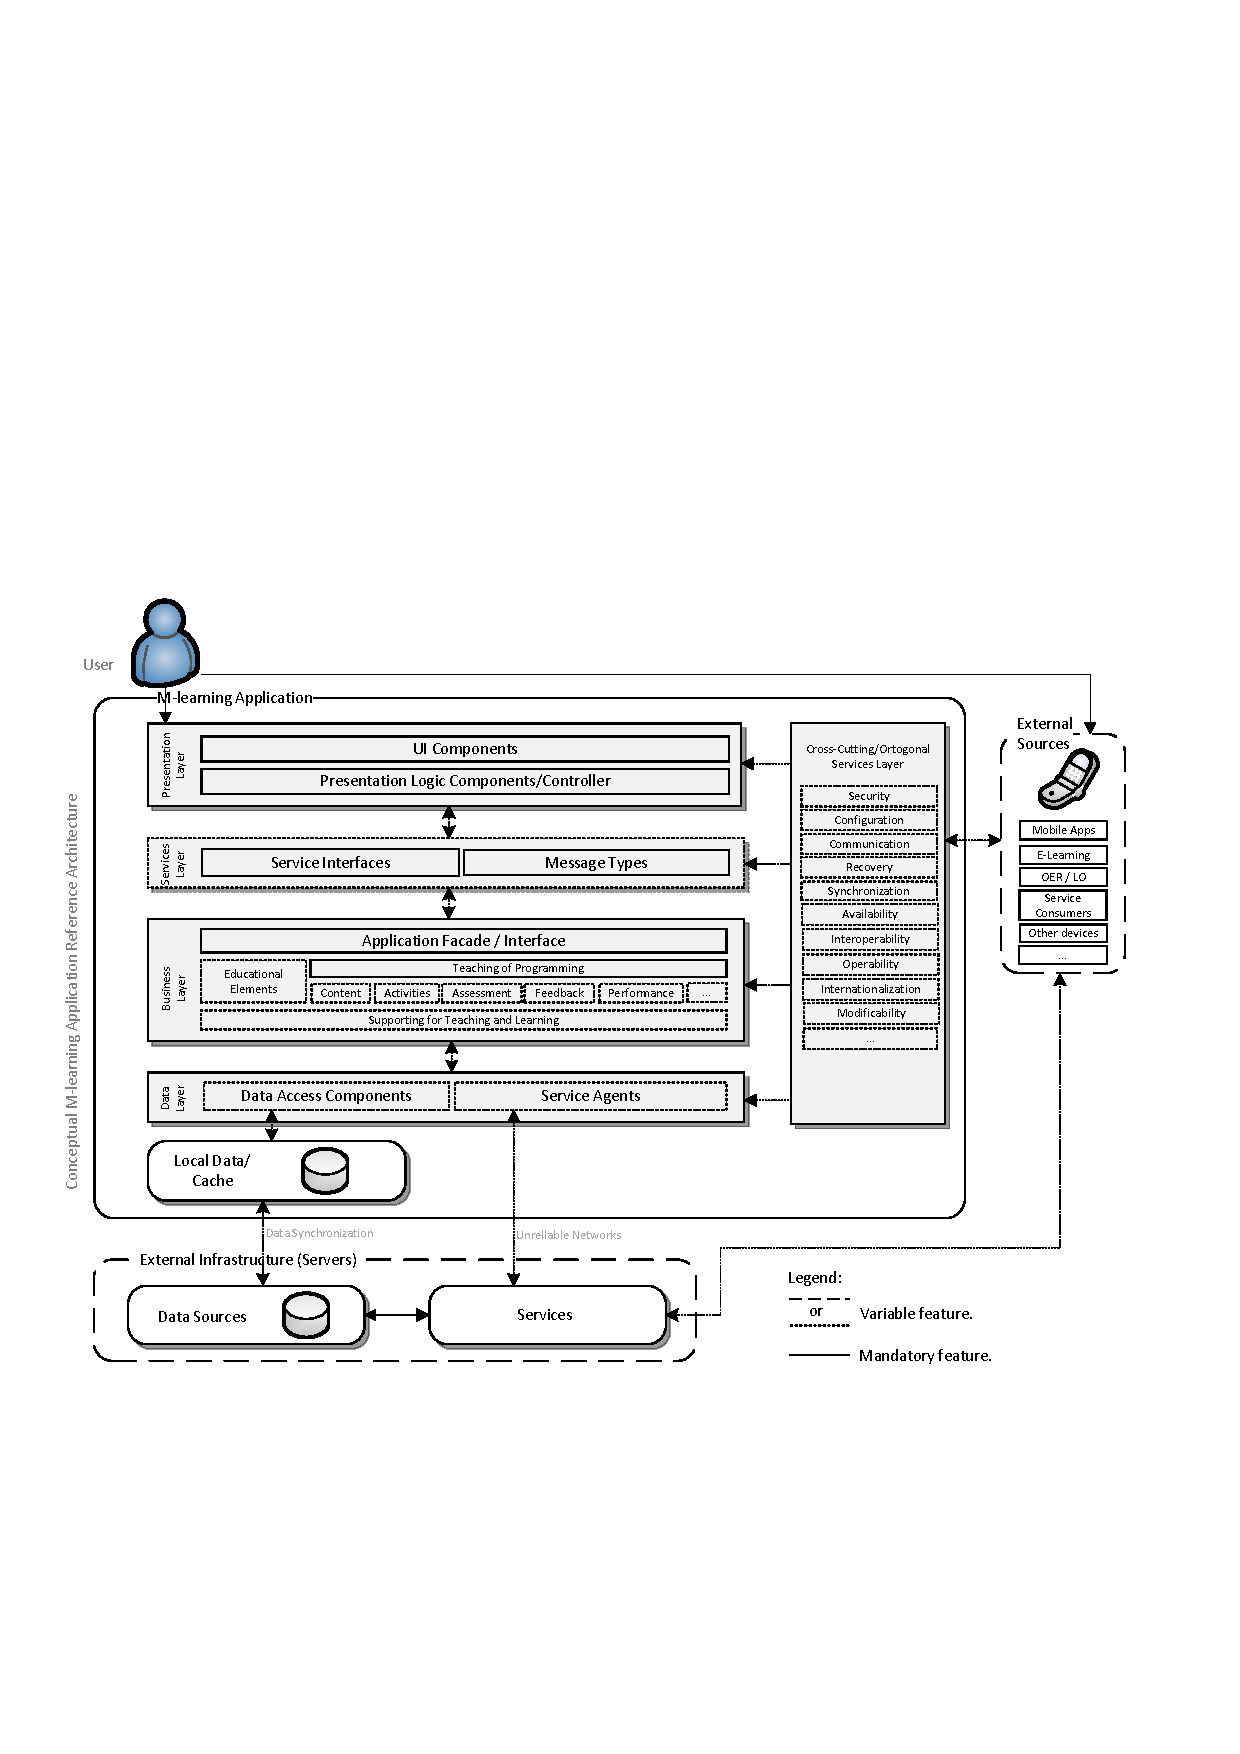
\includegraphics[scale=0.75]{conceptual_old.pdf}
    \caption{M-learning SPL Conceptual Architecture Excerpt \cite{marcolinoarcht2017}.}
    \label{fig:schema}
\end{figure*}

%The three green subprocess (Figure \ref{fig:schema}): Project Management, Domain Requirements Engineering and Domain Design were conducted. This last subprocess was concluded until the logical view through the feature model and the conceptual architecture model. 

The Domain design differs from design of single systems mainly because it incorporates configurations mechanisms into the SPL reference architecture to support the variability of product line, this mechanisms are presented in \cite{marcolinoarcht2017} and are considered in the final SPL solution. Furthermore, it allows the development of an adaptable architecture for future inclusion of new features and designates the reusable parts with no loose of rules for the development of specific applications based on the SPL reference architecture.

However, the evaluation conducted with 31 main stakeholders involved in the process did not consider the industry practitioners. Such stakeholders were from academic area, having know--how in software engineering, programming, m-learning and mobile development. Therefore, a re-analysis in practitioners perspectives is needed before the SPL architecture representation in the development and process views, in which both will be supported by the SMarty approach. The aim is evolve the already evaluated architecture to attenuate possible future problems in development phase.


\subsection{The SMarty Approach}


The SPLE framework designates the adoption of the orthogonal variability model \cite{pohl2005}. However, this model adopt a specific graphic notation, requiring the understanding of the notation to be applied. Additionally, the creation of such models needs specific modeling tools for the conception of them. To minimize the inclusion of a new notation for developers and to easy the process of understanding for industry practitioners, the SMarty approach was adopted in the conception of the SPL models \cite{deOliveira2013, marcolino2013}.


SMarty supports the representation and management of variability in UML models. It supports use case, sequence, class, activity and component UML models through an UML 2 profile, named \textit{SMartyProfile}. UML profile allows an easier integration of their notation in any modeling tool that enables UML profiles import. SMarty also provides the \textit{SMartyProcess}, a set of guidelines that guide users in its application, providing also the support for the detection of (new) features in UML models.

The \textit{SMartyProfile} comprises the following stereotypes: $\ll$variability$\gg$, $\ll$mandatory$\gg$, $\ll$optional$\gg$, $\ll$alternative\_OR$\gg$, $\ll$alternative\_XO$\gg$; $\ll$mutex$\gg$ and $\ll$requires$\gg$. It also has a set of attributes for presenting extra and fundamental information such as the rastreability among the variabilities, the maximum and minimum number of variants, all of them included in an UML comment element.


Finally, other reason for the selection of SMarty was the good results of a set of experimental evaluations, where it was compared the process of identification of variability with UML-based Software Engineering Method (PLUS) and Ziadi et al. approach \cite{marcolino2013, MarcolinoJG14}. Even with a better representation of PLUS method in Class models, mainly by the set of reduced stereotypes, SMarty showed to be the best choice because of its set of guidelines. Moreover, as the approach allows the management of their stereotypes in a profile, the addition of new syntactic elements is facilitated \cite{deOliveira2013}, enabling the constant evolution of SPL core assets.



\section{Evolving the SPL Conceptual Architecture}
\label{sec:spl_project}

The SPL conceptual architecture (Figure \ref{fig:schema}) was evaluated by 31 participants from different areas of expertise, considering the stakeholders' perspective \cite{marcolinoarcht2017}. Based on their profiles, we noticed that all of them are from academic area, implying in a possible bias in the evaluation of the architecture in a industry perspective.

Other issue refers to the results related with \textit{conceptual aspects}, \textit{infrastructure aspects} and \textit{SOA aspects}. Comparing the results with the \textit{general aspects} and \textit{educational domain aspects}, the percentage of results that ranked the architecture as \textit{partially complies} suggests possible issues to be reanalyzed. 

It was also identified the need of evaluating the architecture and the requirements catalog together, since they had been evaluated separately, what could imply on issues such as imprecise understanding of the software solutions. If the \textit{domain design} and \textit{domain realization} SPLE sub-processes are conducted without proper analysis, the cost and effort to re-factor the project and the sub-processes involved could be higher. Thereby, a reevaluation of the proposed architecture was conducted.


\subsection{Methodology}

The methodology applied to support the new analysis of the conceptual architecture follows an industry protocol in which the requirements and needs were deeply analyzed for proposing the architecture.

Such industry protocol involves the process of rigorous analysis of (i) each requirement (functional and non - functional) independently, for the identification of it possible impact and development technique to be adopted; (i) the analysis of set of requirements and possible expect and unexpected behaviors, when combined with other sets of requirements; (ii) architectural designing decisions for each set of requirements and after, for the entire solution; (iv) technical debt issues and; (v) human resources available in the development team and time.

Then the following steps were conducted:

\begin{itemize}
\item the previous architecture model (Figure \ref{fig:schema}) and its publication were analyzed;
\item the requirements catalog was discussed considering the ideas of the first architecture model and the learning and didactic objectives to minimize problems \cite{souza2015} in programming domain considering mobile learning applications; and
\item based on the previous analysis, each package/layer in the conceptual architecture was studied and restructured when necessary.
\end{itemize}

The analysis occurred during one month, where two practitioners from the industry supported the evolution of the model. Both have an average of eight years of expertise in mobile development in industry. One of them have also expertise in software product line, three years, and the other one in development of hybrid applications, five years.

It is highlighted that the number of practitioners is small, but considering the availability and the reality of Brazilian academy agreements with software industries, this interaction, even in with a small participants, allows the identification of possible lack of know-how in academic perspective, where the theoretical knowledge is bigger than the practice. Finally, it is also emphasized that the participants also collaborate with the development of the UML models with SMarty.

\subsection{Discussions and Evolved Conceptual Architecture}

After the execution of each step previously discussed, the conceptual model was updated as shows Figure \ref{fig:schema2}.


\begin{figure*}[!ht]
    \centering
    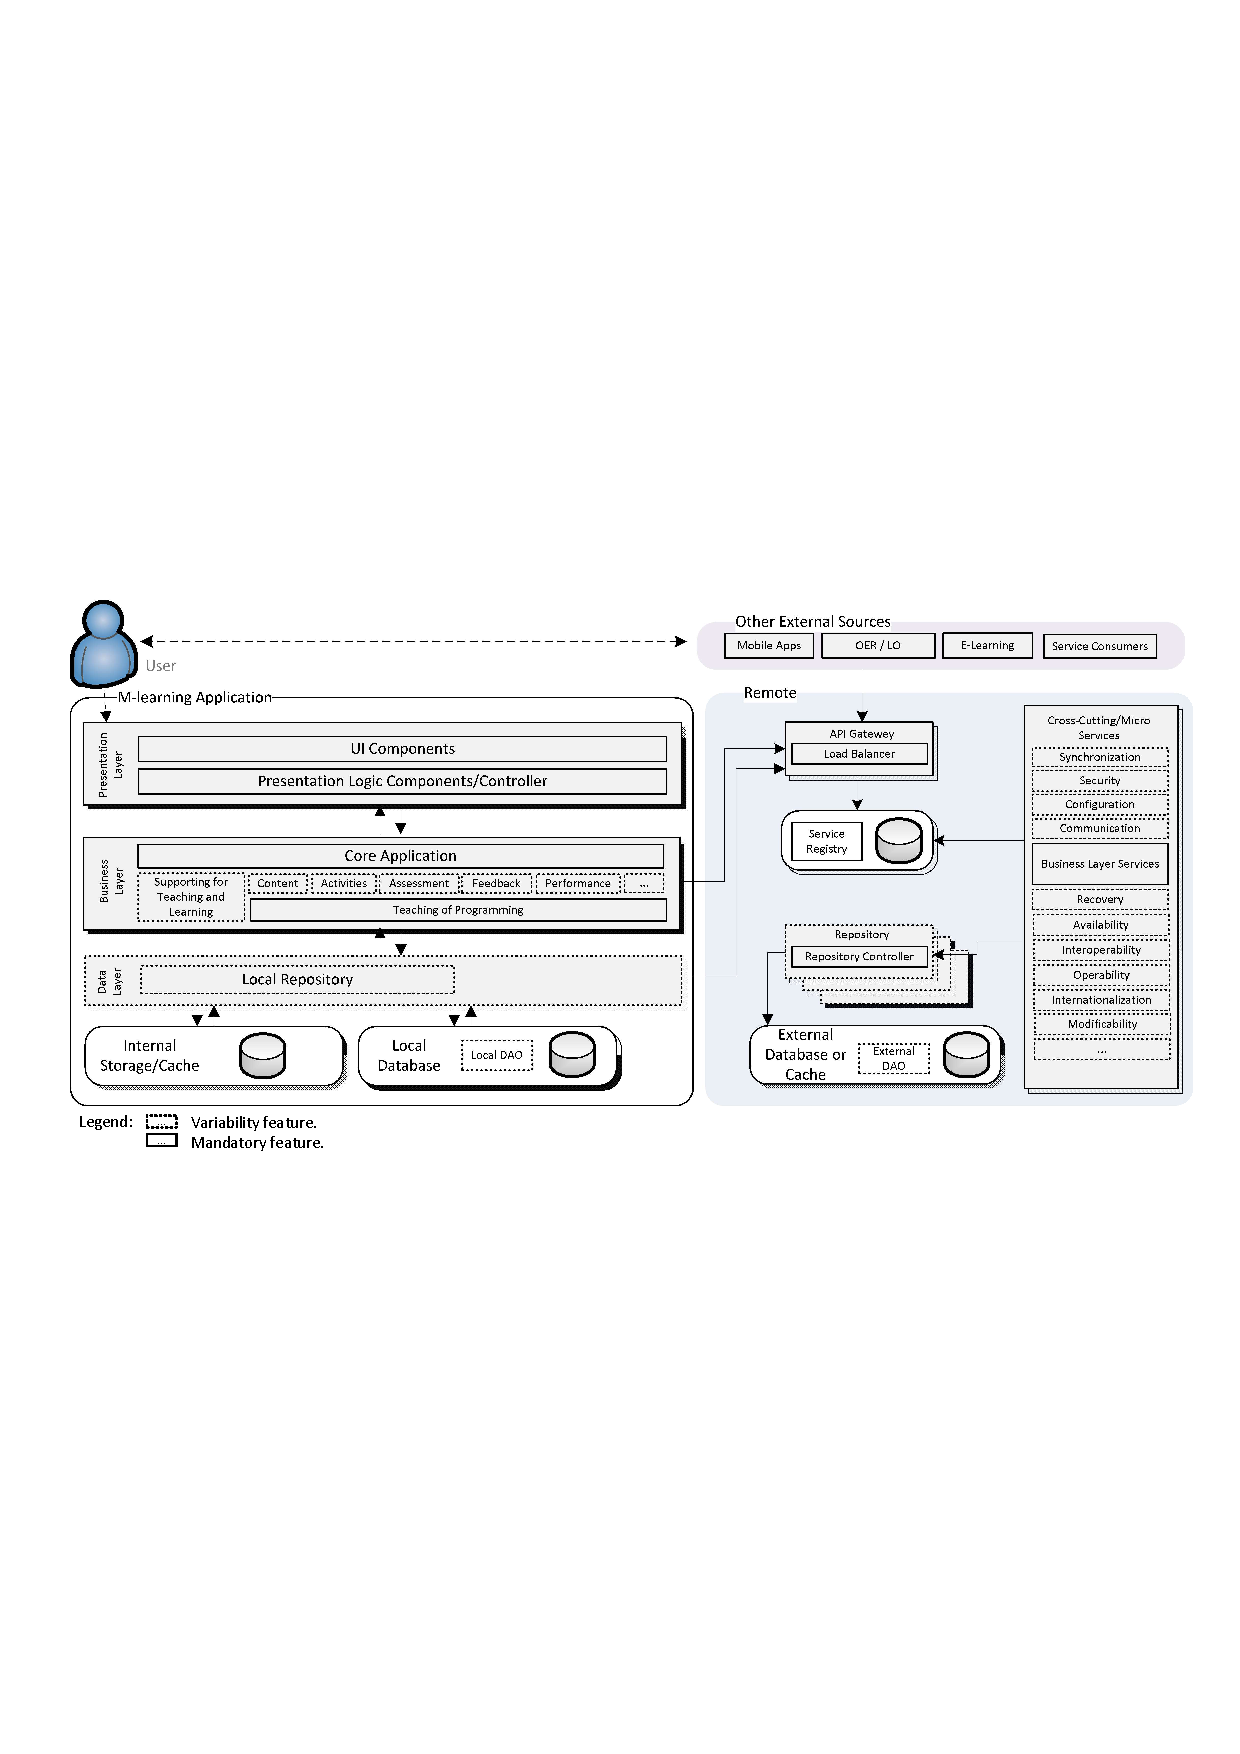
\includegraphics[scale=0.90]{archv7.pdf}
    \caption{Updated M-learning SPL Conceptual Architecture.}
    \label{fig:schema2}
\end{figure*}

\textit{Domain Engineering}, \textit{Application Mechanism} and \textit{Application Engineering} do not changed (Figure \ref{fig:schema}). All of them continue with the same roles and sub--processes, with the exception from the way in which the applications are generated. This change implies in most of the changes in the m--learning application architecture.

For the user, the \textit{application mechanism}\cite{marcolinoarcht2017} will work in the same way: the user answers some questions or selects the desired features and the support mechanism generates the application for download. However, with the updates, the choices made by the users will be stored in a database (or metadata files) and will be considered for delivering an application instantiated with only the selected features. So, if the institution privilege is considered, only a set of features allowed for it will be available for the users' institution. This software architecture strategy is called multi--tenancy.

The mult--tenancy architecture refers to an architecture in which a single software solution is executing on a server, serving multiple groups of users who share common access in such instance of software. Each of these groups is called tenant. Looking at cloud computing models, the multi--tenancy approach is perfectly adherent to Software as a Service (SaaS) \cite{krebs2012architectural}.

The change in the application mechanism implies in a delivery of a complete application instance (presentation and business layers), no matter the selected features. However, at the end, the application will solve its variabilities in execution time based on the set of selected features, providing only features and services related to the current user, the owner of the configuration defined in advance.

In the multi--tenancy proposal, the code and database packages are installed on a single server, simplifying the release and scalability processes \cite{krebs2012architectural}.

At this point, many concerns arise:


\textbf{Q1 -- Why was this decision made?}

Imagine the hypothetical scenario where a teacher generated an application for two classes to be used in one semester. After finished the period, he receives in the next semester four more classes, but now he wants to use the application with a new feature, not selected in the previously semester. Until now there is no problem. He can generate another application and use it with his new classes but, and the data from the other application? Additionally, if the teacher decides to change his choices for the application in the middle of semester, he will need to create a new application and re--install each student's application. Furthermore, if the new configuration is not concise with the previous features -- in a software product line constraint perspective -- teachers and their students will not be able to correctly use the application with the new changes. 

A final issue is the number of applications to be controlled based on several teachers and classes in the same institution. Data for the educational administrator will be always broken in parts, making the process to manage and to improve the learning and teaching processes difficult, mainly by each specificity of the applications. It is highlighted that this requirement was not change, just new considerations were made, allowing a deeper understanding of the features, besides, this is only one of several implications that were identified, leading to the proposed changes.




\textbf{Q2 -- Do these changes not imply in significantly changes on the functionality of the applications?}

Yes, mainly about the connection-dependency. Adopting multi--tenancy implies in a connection, since this connection will be required for the presentation layer shows only the features selected for the current user. However, cache and local database can be used to allow the use of the application when a connection is not available, mainly when a mobile device is the platform in use. Such usage is the reason for a new update in the architecture: the adoption of repository pattern, later discussed in this section.

\textbf{Q3 -- Which trade-off may these types of application have?}

\begin{itemize}


\item \textbf{Positive factors:} one instance in a server for multiple users, centralizing scalability issues and simplifying the release management.

\item \textbf{Negative factors:} Larger development effort, mainly to maintain and to use per--tenant data allowing the customization of the applications. Furthermore, multi--tenancy increases the risks and impacts inherent in applying a new release version. As there is a single software instance serving multiple tenants, an update on this instance may cause downtime for all tenants even if the update is requested and useful for only one tenant \cite{krebs2012architectural}.

\end{itemize}

%There are other positive and negative factors but those are highlighted considering its integration in an SPL for the development of mobile learning applications in a fist instance.

Based on the adoption of multi--tenancy, a new challenge appears: guarantee the correct execution of applications in mobile devices in areas where network connection is not available. For this, as mentioned in \textbf{Q2}, the repository pattern was adopted as a solution in the SPL architecture proposed. Although, before the understanding of this pattern, it is important to make an observation related to the pedagogical and didactic concern: the constantly feedback in applications.

According to Marcolino and Barbosa \cite{marcolinoarcht2017}, there is a problem in the given feedback in mobile applications for the teaching of programming. As such applications generally support informal than formal learning, feedback features are given only for one of the categories of the users, teachers or students. Thereby, the need of a more concise feedback to support students to learn by themselves and to notify teachers about the students' performance is a mandatory pedagogical and didactic feature to support formal learning. The feedback allows the improvement of the curricula, changes on didactic strategies adopted in classroom, changing on teaching topics and other improvements \cite{marcolino_catalog2016}. Thus, the adoption of a mechanism to store and retrieve the data of the learning process is fundamental, meeting the need for the adoption of mechanisms to enable it, as the repository pattern does.

The repository pattern avoid the directly access of data from the business logic layer, services or other entities, reducing the duplicate code, weak types of business data, the difficulty in centralizing data from cache and several data bases and, the inability to easily test the business logic \cite{repository}. The pattern manages several data repositories, common in a microservices architecture and it also enables caching and storing data in mobile applications. Based on these benefits, the repository pattern was selected to deal with the multi--tenancy concerns, integrating a DAO (data access object) strategy when convenient, and easing the manage of data from the microservices -- other update in the proposed SPL architecture.

The repository is shown in Figure \ref{fig:schema2}. It is available in two perspectives, directly in the client application or in the server side. The \textit{local repository} can realize the persistence through internal storage, i.e., private data in the device memory; or in local database, i.e., structured data in private database and; with network connection, i.e., calling a microservice. On the other hand, the repository on the server side is used by the microservices only, and realize its persistence through a external storage, i.e., a database or cache \cite{repository}.

Among other benefits encompassed with the adoption of the repository pattern, we highlight that: (i) they can adopted different persistence strategies for different contexts, such as relational databases, non-relational databases, cache and services; and (ii) applications can adopt managers for easing the integration and encapsulation of the dependencies strategies.


Finally, the last update made was the adoption of microservices concept, which integrates the SPL proposal for the development of applications as a SaaS \cite{Newman:2015:BM:2904388}. 

The adoption of mobile learning applications has several benefits (see Section \ref{sec:background}). However, the management of data, the availability of new content, learning activities and other elements presented in a learning environment though the reduced mobile screens and its native keyboard may not be a good way for conducting such tasks. In this perspective, providing different paths of access to those functionalities in different platforms can improve the user experience and, microservices support this strategy.


\begin{figure*}[!ht]
    \centering
    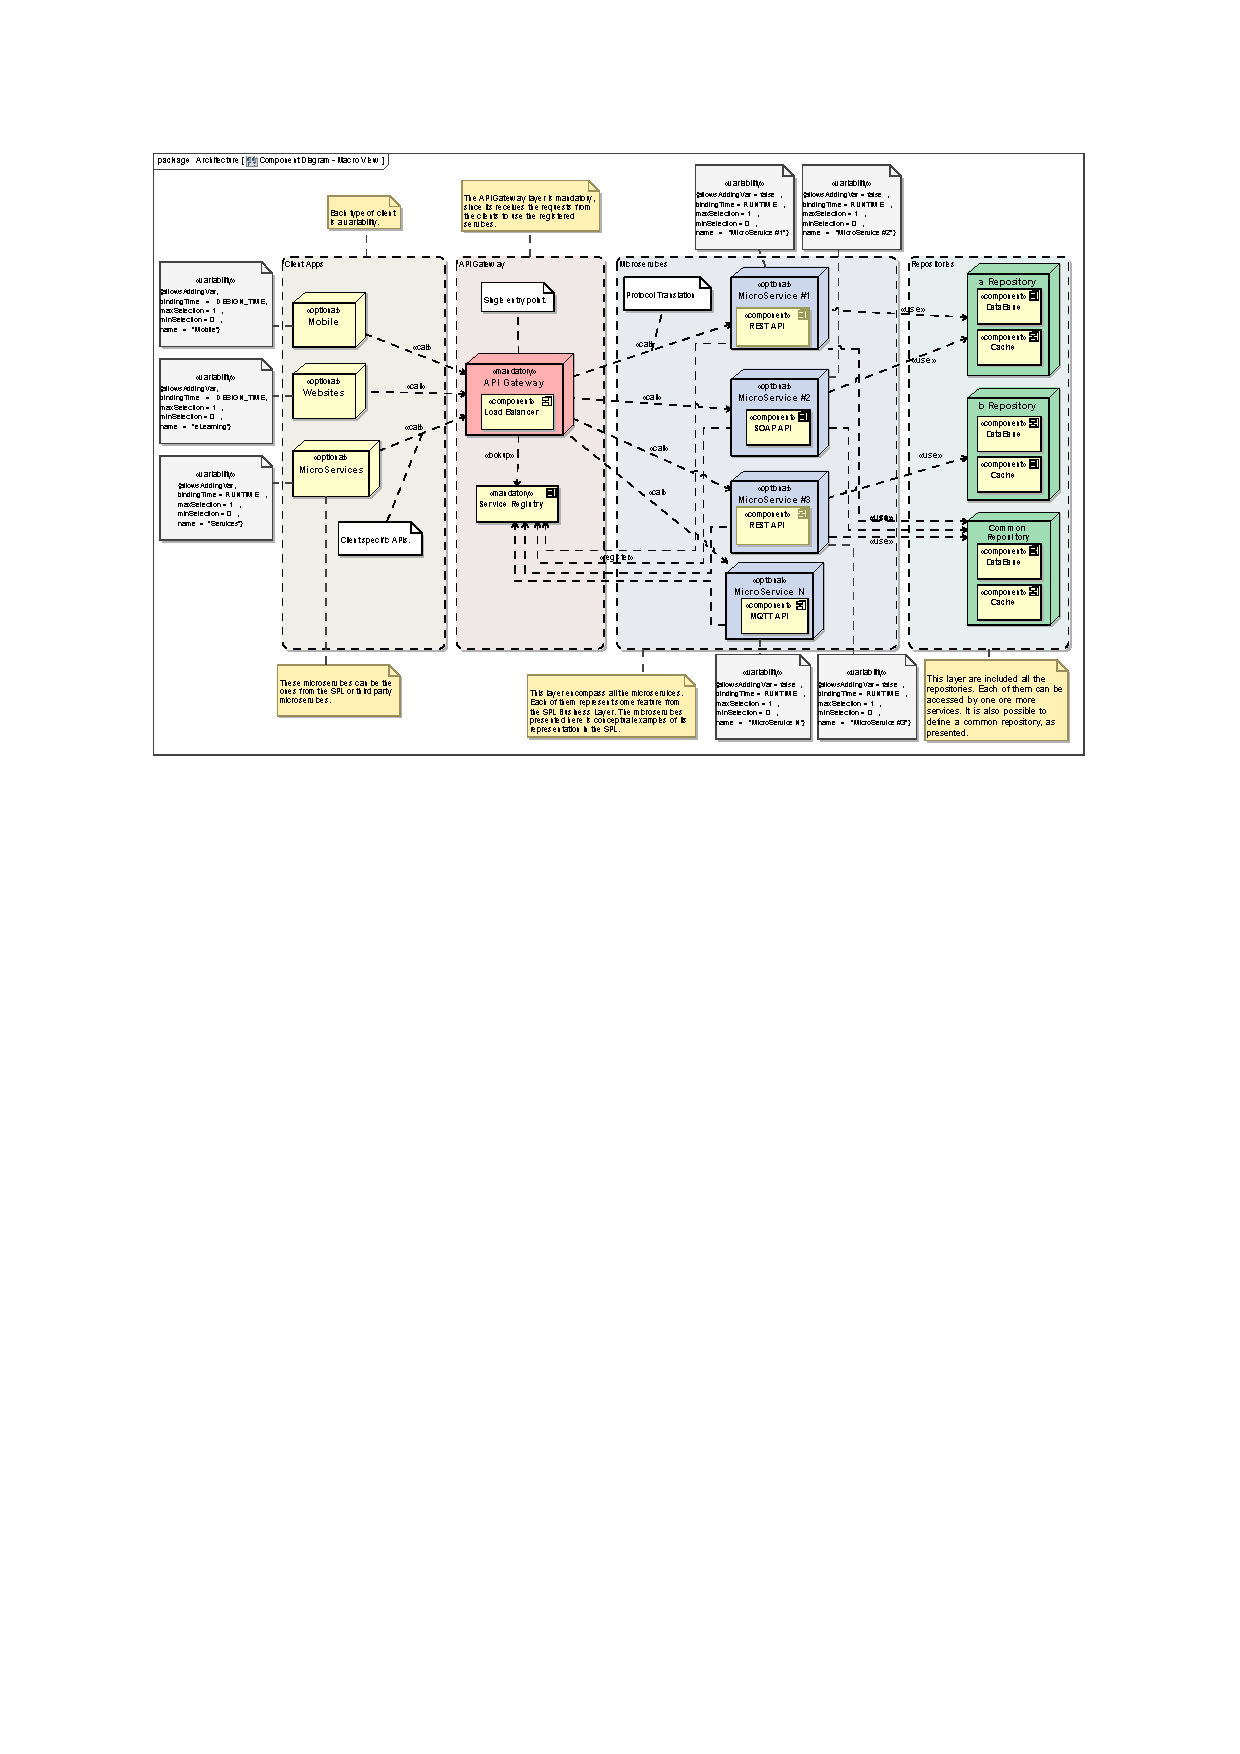
\includegraphics[scale=1.00]{component.pdf}
    \caption{M-learning SPL Component Model.}
    \label{fig:comp}
\end{figure*}

Microservices allow the use of different platforms and technologies as consumers of them. The responsibility is uncoupled from the business layer, which has only the function of accessing the microservices available on one or more servers and providing for the presentation layer such functionality. Looking at the SPL concept, the microservices meet and facilitates the process of management and definition of variabilities. Microservices provide a set of fully uncoupled services, but highly collaborative. Each service implements a set of narrowly, related functions. For example, an application might consist of services such as the order management service, the customer management service, etc.

Services communicate using either synchronous protocols, such as HTTP/REST (Representational state transfer), SOAP (Simple Object Access Protocol), or asynchronous protocols, such as AMQP (Advanced Message Queuing Protocol) and MQTT (Message Queue Telemetry Transport). Also, they can be developed and deployed independently of one another \cite{Newman:2015:BM:2904388}. As each service has its own database, the data consistency is improved. Add a data management standard, such as repository, and you'll have an even more robust solution. And, considering the multi-tenancy architecture, just the features selected in advance will be available and visible for each tenant/user.

Also in Figure \ ref {fig: schema2}, other difference from the first model is clear: the relation between \textit{other external sources} with the application. This goes to meet what was discussed about the multi--tenancy and microservices. These external sources will benefit from these adoptions, since its relation with the \textit{API Gateway}, its \textit{load balancer} and the \textit{service library} will allow the consumption of the microservices by other platforms or even by other applications, improving the reuse of features not dependent from the domain of the line.

The extra \textit{service layer} was removed and the \textit{core application} component replaced the \textit{application facade/interface}. Now, the \textit{business layer} has a relation with the \textit{API Gateway}, which balances the requests among the different tenants and applications to the microservices which are, in their turn, registered in a data base managed by the \textit{service registry}. Every microservice that reflects a feature in the SPL and is available to be selected by users, has a register entry that is visible by the \textit{service registry} and available by it for the \textit{API Gateway}, responsible to redirect each requisition received from the \textit{business layer} or \textit{external sources} for its respective microservice.

Among other benefits encompassed with the adoption of microservices, we highlight that: (i) they are independent; if one fails or goes to maintenance, the others will continue available; (ii) they can be implemented adopting different technologies; (iii) they can have one or more repositories; and (iv) they can be encapsulated and works only with the complexity from the business domain, easing the development, since the complexity is distributed among such domains.

Some concerns also emerged with its adoption: (i) it is hard to separate business domains, but for our SPL this difficulty does not occur, since the mentioned m-learning requirements catalog solve this concern; and (ii) the deploy of several microservices and the hardware maintenance need more efforts than the development of monolithic systems.


We also highlight some API Gateway benefits: (i) it is adopted as a facade layer with the objective to facilitate the clients' accesses to the microservices; and
(ii) it is an ``intelligent'' layer that can balance the load of number of requisitions and the caching information.
 
On the other hand, one concern is the disadvantage in the creation of a single point of failure.



Therefore, with the macro view of the conceptual SPL architecture updated, the \textit{domain design} sub-process is retaken Its artifacts models are presented and discussed next.







\section{SPL Architecture with SMarty}
\label{sec:spl_smarty}

The SPL methodology differs from the development of singular software by the postponement of project decisions. The features are included in the software by convenience and the need of stakeholders. In the proposed SPL, the variabilities are concentrate in the \textit{business layer} features \cite{marcolinoarcht2017}. 

The integration of the teaching of programming domain, mobile platform and teaching and learning processes presents several features. The most of them need to be combined to provide a richer learning environment, allowing the achievement of the educational objective. The several features considered in the proposed SPL come from the analysis of 81 applications and software systems in the programming domain \footnote{\url{goo.gl/EvzUpB}}. Consequently, the catalog was represented in a feature model, depicting the relation among features, variabilities, variation points, variants and their constraints. As previously mentioned, SMarty was selected to represent this in UML diagrams. 



Among the \textit{domain design} sub-processes, the \textit{logical view} is represented through the feature model \cite{LindenSchmidRommes07}. The \textit{development view} can adopt the package diagram, component and class diagram. Figure \ref{fig:comp} shows the component model of the SPL.  



\subsection{Component Architecture}

The component diagram depicts how components are wired together to form larger components or software systems. They are used to illustrate the structure of arbitrarily complex systems\cite{Pressman:2015}. The SPL representation has four layers: \textit{client apps}, \textit{API gateway}, \textit{microservices} and \textit{repositories}.

\textit{Client Apps layer:} this layer shows the apps, platforms, websites, services or any potential consumer of the microservices. The main clients considered in the research are \textit{mobile apps}, followed by \textit{websites}. These clients have just the view and controller of the application. All the business logic is inserted in the microservices. However, they are the main way to wire together all the desired features by the tenant/user, previously selected in the \textit{application mechanism}. Additionally, all the clients are considered optional variabilities, since they may or not be part of the SPL. 

\begin{figure*}[!h]
    \centering
    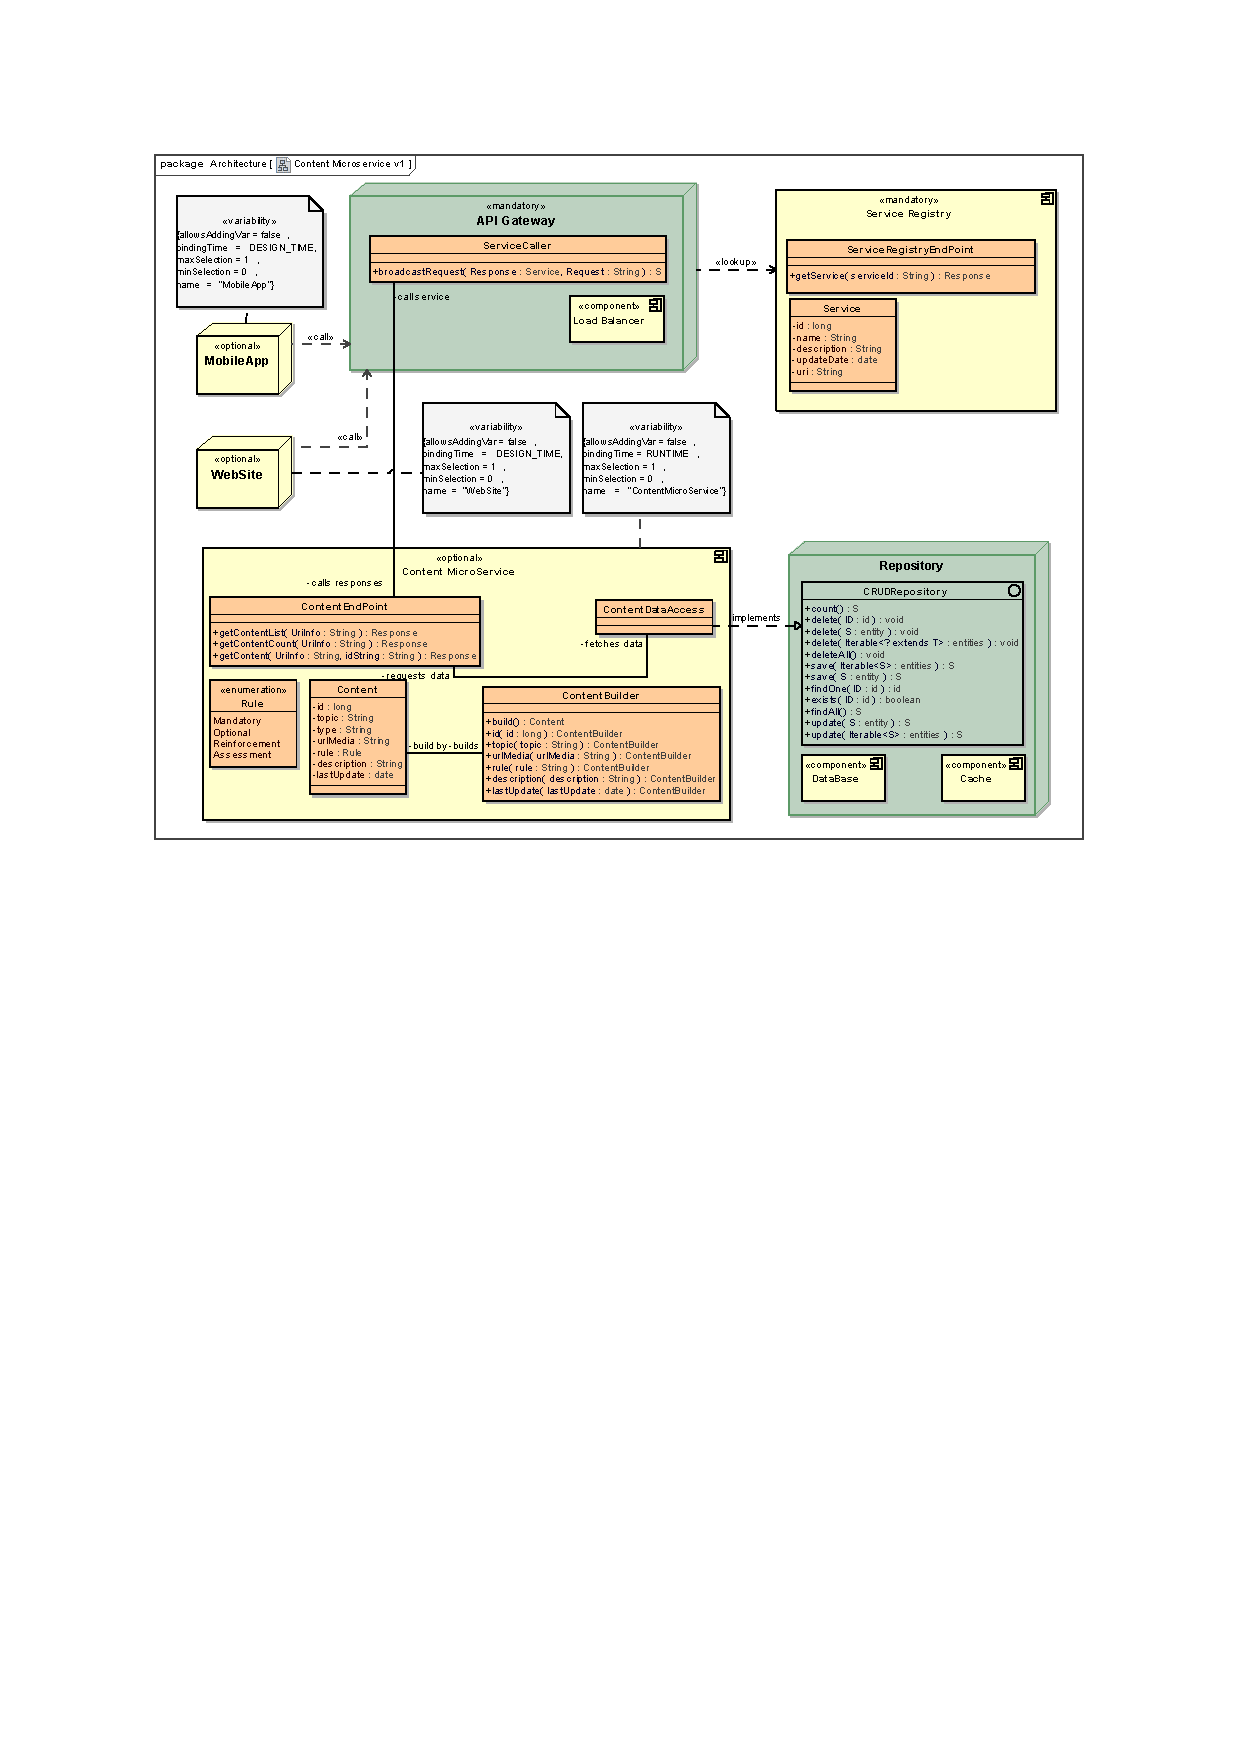
\includegraphics[scale=1.00]{content.pdf}
    \caption{M-learning SPL Content Microservice Class Diagram.}
    \label{fig:class}
\end{figure*}



In the representation, the clients are tagged as $\ll$optional$\gg$ and each one has a UML comment which depicts additional information about them. Those variabilities are solved in design time. Each instance of client calls the \textit{API Gateway} node from the next layer.





\textit{API Gateway:} this layer identifies the available microservices registered in a data base through the mandatory \textit{service registry} component. The \textit{API Gateway} node, also mandatory, looks up for the microservice requested by the client in the \textit{service layer}. If the microservice is found, the requisition is broadcast for the respectively microservice in the next layer. Additionally, the \textit{load balancer} observes the behavior and quantity of requests from the clients, balancing the load of data traffic and ensuring that all the requests will be answered, controlling them in a row. This component is also responsible to increase the server resources; in other words, it provides the elasticity of the cloud resources \cite{Pressman:2015, Newman:2015:BM:2904388}.




\textit{Microservices layer:} this layer encompass all the microservices, although each one can stay hosted in different servers. The microservices has specific functionality, from non-functional to functional ones and each represents the features depicts in the feature model. They are instances of each selected feature in the \textit{application mechanism}. The model presents four samples of services. Everyone has a component which express the type of supported protocol and, based on this protocol, each one receives requests directed by the \textit{API Gateway}. Still in this layer, each microservice is tagged as optional variability, but following the feature model, some of them will be represented as exclusive ($\ll$alternative\_XO$\gg$) or be mutually exclusive among the other microservices selected. For instance, educational activities can be available following a fixed order or be performed by convenience, therefore, these two features of the availability of educational activities follow the SPL mutually exclusive constraint. On the other hand, there are features that require others, such as the learning monitoring and performance, that needs feedback features to support both teachers and students.

Other behavior on the microservice layer is the possibility for the microservices to do calls among them, when it depends on the process of another microservices, removing the needs of processing from the client. These calls among the microservices is also performed by the API gateway.




\textit{Repositories Layer:} in this layer all repository structure is presented. They can be in different servers and, in some cases, they are not mandatory for some services. The repository is responsible for the management of the persistence process, providing interfaces in DAO model, if convenient, for enabling the access of the data in their registered data base. They also coordinate the cache usage.




\subsection{Architecture Class Diagram}





The next architecture artifact from the SPLE framework is the class diagram (Figure \ref{fig:class}). For this representation, as each microservice represents a feature, or a small set of them, the class diagram was divided in one representation for each existing artifact. This decision was made based on some issues, particularly: (i) the reduced number of developers, (ii) the reduced time for the development of each feature before its development, (iii) the facility to manage each diagram of the architecture as an artifact from the SPL core asset; and (iv) the the extreme programming (XP) agile process \cite{Beck:2004:EPE:1076267} with the test driven development (TDD) \cite{Fraser:2003:TDD:1763875.1763973} adopted for the conduction of domain realization and domain testing SPLE sub-processes (an investigation about this adoption will be conducted in order to provide evidences of the possible benefits in SPL context) .




%As consequence of the reduced number of developers and the big number of features to be developed, a questionnaire has been applied with programming teachers to identify the priority of the features.  Based on the results, a set of candidate features was selected in the conduction in the first iteration of the domain realization and testing sub-processes. Furthermore, based on the number of developers, the adoption of an agile methodology was included in the SPL project, the extreme programming (XP) agile process \cite{Beck:2004:EPE:1076267} with the test driven development (TDD) \cite{Fraser:2003:TDD:1763875.1763973}.




%Extreme programming process is iterative and incremental. It is an agile process because it emphasizes the communication and feedback among the project team. However, the main motivation to its adoption was the frequent iterations and its short releases, which eliminates defects earlier, reducing costs and meeting the objective in the adoption of microservices: the fast development of features, the fast availability for the customer and the concentration of efforts in short releases.



%\begin{figure*}[!ht]
%    \centering
%    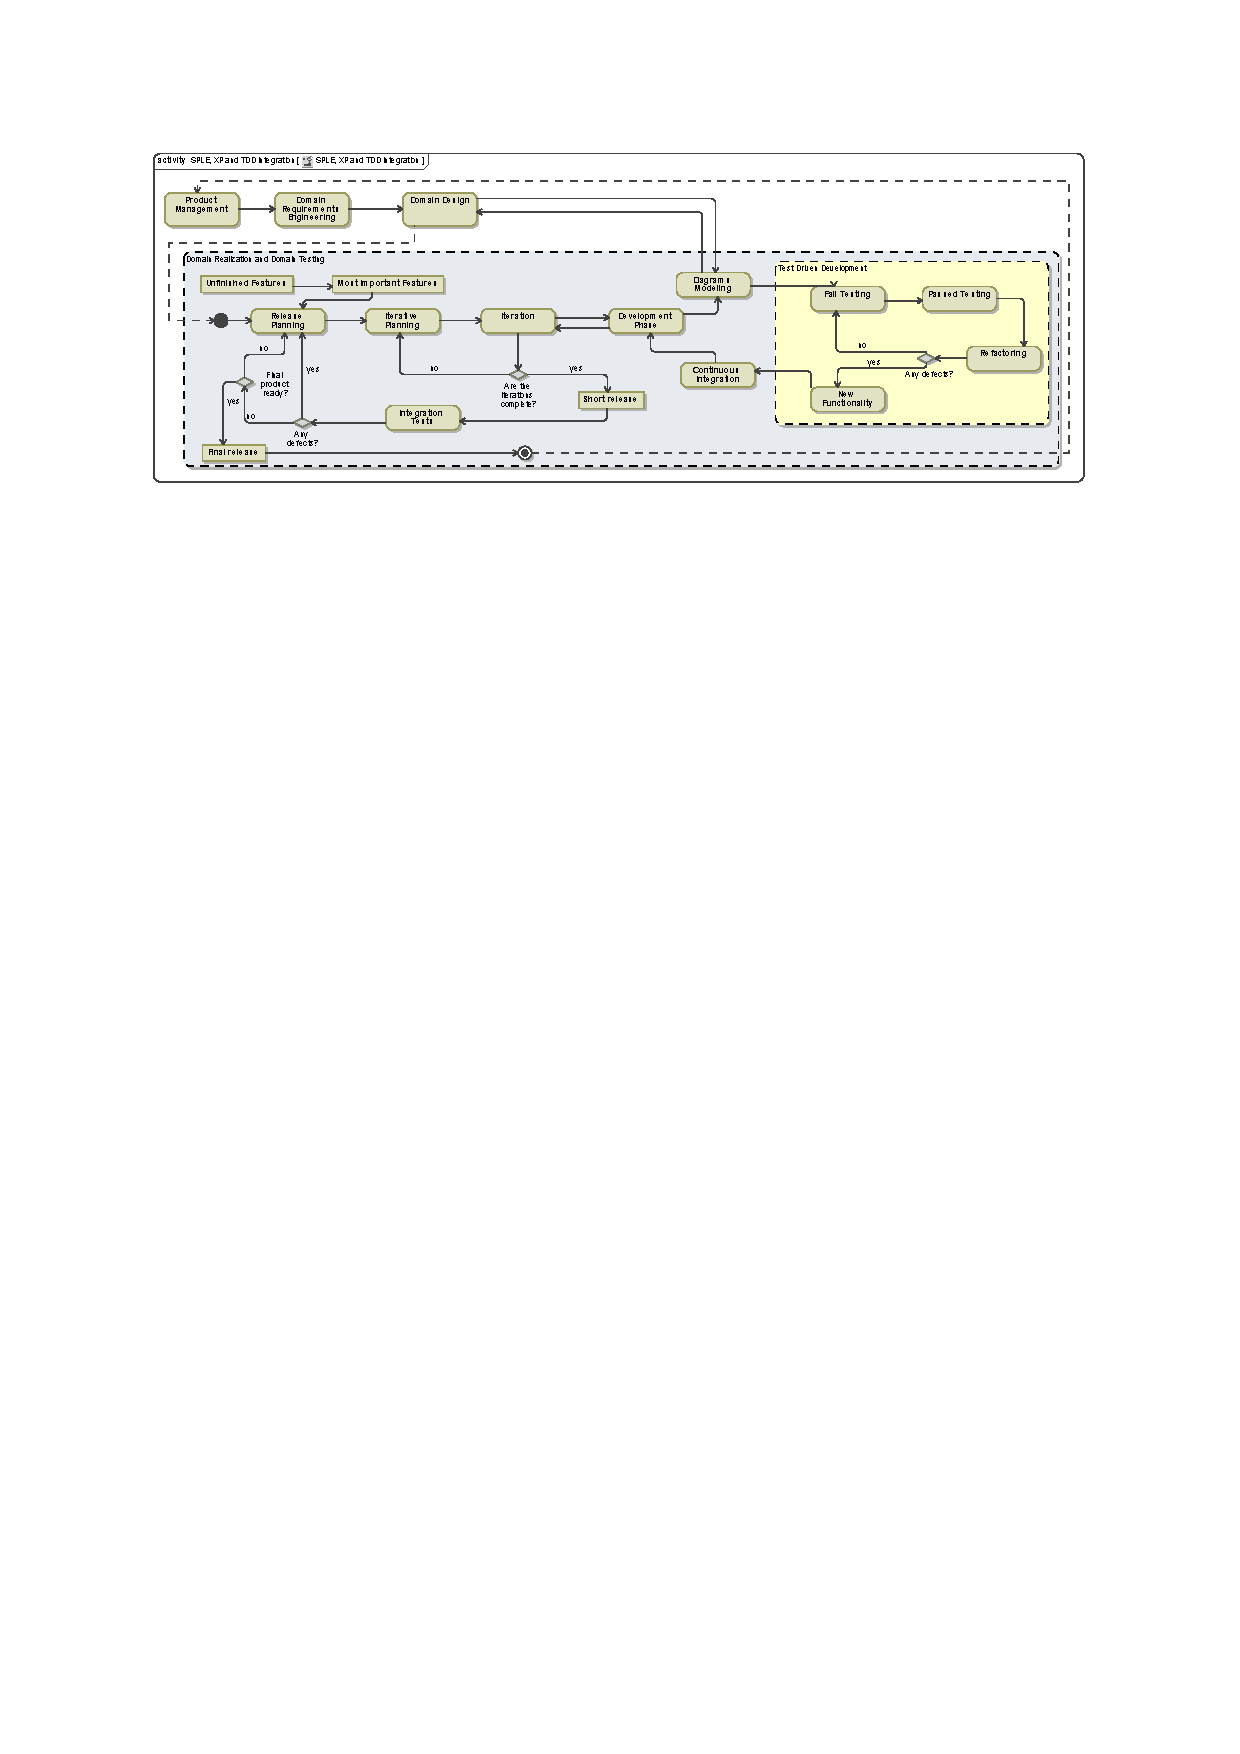
\includegraphics[scale=1.11]{activity.pdf}
%    \caption{Activity Diagram with the Integration of SPLE, XP and TDD.}
 %   \label{fig:activity}
%\end{figure*}


%In this perspective, to integrate and to agile the domain test realization, TDD was adopted together with XP. Such development technique has its base on the repetition of short cycles. Each development of a new functionality starts from the definition of a test. This test must fail because it is wrote before the functionality be implemented; if it fails, the proposed functionality or improvement is obvious. To write a test, the developers may understand the specifications and requirements of the functionality. It can be done through uses cases or use stories that cover the requirements and the conditional exceptions. In the context of the line, the requirements catalog with the feature model and its constraints were considered. This is the main difference from the process of writing unit tests after the code is ready. It keeps the focus of the development in the requirements before the coding, which is a subtle but important difference.

%After the definition of the test that must failed, the next phase is to check if the new test does not bring errors. In other words, this phase tests its own test. Next, the test must failed by the expected reason: the functionality has not been developed yet. In the next phase the code which must pass in the test is developed. 

%The developed code can be wrote presenting some problems or did no pass in a elegant way, since the next step will be improved it. The aim is to write a code that pass in the test. If the developed code passes in all the tests, it means that all the requirements were considered in the code, starting the final phase of the TDD: the coding refactoring. In this phase, the code is improved, removing redundant code and verifying if it still passes in the tests cases previously checked. In this phase, the modeling of the class diagram of such functionality is performed and the cycle is started again. With the development of a new functionality, the continuous integrity has a fundamental role to provide reversible points, once a union of functionalities could generate errors, when integrated.

%After the TDD cycle, the XP cycle continues. The functionality released is analyzed in a integration test and, if passed, the release can generate the expected product or be stored in the core asset to be integrated after, with other functionality to be developed.


%Figure \ref{fig:activity} depicts an activity diagram that summarizes the integration of the XP agile process and TDD technique tasks with SPLE framework sub-processes.


Figure \ref{fig:class} shows the content feature microservice represented in a class diagram. The diagram considers two instances of clients: an \textit{MobileApp} and a \textit{WebSite}. Both calls the content \textit{API Gateway} which look up in the \textit{Service Registry} to identify if the requisition for such microservice can be answered. For this, the respective called microservice need to be register on the queried data base and be identified with the support of a \textit{repository}. With the identified service, the \textit{API Gateway} can localize the service through its \textit{uri}, executing the request that comes from the customer and returning to it the retrieved content data being presented in their app interface through the controller of content and its communication with the presentation logic layer.

Three variabilities are represented in the class diagram. The two clients, where both are solved in design time; and the content microservice, that is solved in runtime. The content microservice is considered a variability because some learning applications can be developed only to provide activities for the students, not being mandatory for every application. The difference among the binding time of the variabilities is related with the type of variability. The clients need to have its presentation and business logic layers developed before, since they will consume the available microservices accordingly to the permission of features selected for users on the \textit{application generation mechanism}. The availability of the microservices, in turn, will occur in runtime. All microservices will be available for the client applications, although only the ones that the user logged in the application have permission or were selected to their users will be visible and can be used.




\subsection{Lessons Learned}

Based on the tasks and decisions made on this research, the two main lessons learned were:

\begin{itemize}
\item Evaluate the requirements catalog and after, the first conceptual model architecture without a integration of both could be resulted in future problems in development phase. This was made based on the order of research phases and this threat was mitigate based on the practitioners analysis.
\item Microservices improve the reuse and, in some cases, can be adopted in other software programs independently of the domain. Additionally, the reduced size of functionalities expressed on them enables the creation of a greater number of configurations of application. In this perspective, other microservices can be easier integrated to our solution and even, our microservices can be reused in other contexts. However, the evolution of the line will need more attention, since the communication among these microservices requires more efforts and tests to guarantee that they will work properly.



\end{itemize}


%It is also important to highlight that the integration of the XP process and TDD technique in the SPLE framework needs to be better investigated in order to provide evidences of the possible benefits when considered to create an infrastructure for the development of mobile learning applications for the teaching of programming. This is a topic for future research.





\section{Conclusions and Future Work}
\label{sec:conclusions}

In this paper we discussed the evolution of a conceptual SPL architecture for the development of mobile learning applications for the teaching of programming based on the analysis of practitioners from the industry. The first model considered only theoretical and academic views for its evaluation. To provide a more real industrial perspective, two practitioners were integrated to our research, giving contributions to the improvement of the project.

Based on the evolved model, the component architecture diagram was presented. The model encompasses the multi--tenancy concept, microservices and repository pattern. Furthermore, the content feature was represented with UML diagram and the SMarty approach.

All the decisions and models proposed lead to a possible solution for some problems faced on the domain of teaching and programming through mobile learning applications. The discussions presented also allow the adoption of these decisions in other projects which need to deal with several educational features and short releases, besides to promote the reuse of these features.

Our next steps are the finishing of the analysis performed with teachers of programming to define our first set of features to be developed and integrate the core asset of the line. Additionally, the proposed integration of XP and TDD needs to be carefully registered to allow the identification of its positive and negative impacts on the development process.



\section*{Acknowledgment}


The authors acknowledge the Brazilian funding agencies (CAPES (DS-8907173\/DT), FAPESP and CNPq) for the financial support provided to this research.





\bibliographystyle{plain}
\bibliography{references} 

\end{document}


